\chapter{Lab 1 - Introduction to the Digilent Analog Discovery}
\section{Objective}

The purpose of this laboratory is to familiarize students with the Digilent Analog Discovery and its associated software suite. 

%
%The Digilent Analog Discovery offers variety of test bench equipment in a small package that can be used almost anywhere. While the hardware and its associated software package are powerful, practice is required to use it properly. 
%
%This lab is unique because there is no lab report but in its place is a lab practical exam where the lab instructor will ask the student to generate a variety of signals and display them appropriate on the scope to probe that they understand the basics. 

%%%%%%%%%%%%%%%%%%%%%%%%%%%%%%%%%%%%%%%%%%%%%%%%%%%%%%%%%%%%%%%%%%%%%%%%%%%%%%%%%%%%%%%%%%%%%%%%%%%%%%%
\section{Materials}
%%%%%%%%%%%%%%%%%%%%%%%%%%%%%%%%%%%%%%%%%%%%%%%%%%%%%%%%%%%%%%%%%%%%%%%%%%%%%%%%%%%%%%%%%%%%%%%%%%%%%%%

\begin{itemize}
	\item Laptop with Waveforms required
	\item If using a Macbook with the M1 chip (2020 or newer Macbooks) a parallel booting system is required
	\item Digilent Analog Discovery
	\item Breadboard
	\item Wiring kit
	\item Lab parts kit
	\item Multimeter
\end{itemize}

%%%%%%%%%%%%%%%%%%%%%%%%%%%%%%%%%%%%%%%%%%%%%%%%%%%%%%%%%%%%%%%%%%%%%%%%%%%%%%%%%%%%%%%%%%%%%%%%%%%%%%%
\section{Introduction}
%%%%%%%%%%%%%%%%%%%%%%%%%%%%%%%%%%%%%%%%%%%%%%%%%%%%%%%%%%%%%%%%%%%%%%%%%%%%%%%%%%%%%%%%%%%%%%%%%%%%%%%

The Analog Discovery combines a variety of tradition test bench tools in to at simple embedded device that fits in the palm of your hand. This lab focuses on bringing students up to speed on how to use the variety of tools associated with the Analog Discovery. 

There are a variety of tutorials and how-to examples on getting started with the Analog Discovery and its associated software. A good place to start is the Digilent Getting Started Guide: \url{https://reference.digilentinc.com/learn/instrumentation/tutorials/analog-discovery-2-getting-started}. There are also a variety of tutorials for working with the specific tools: 

\begin{itemize}
	\item Using the Waveform Generator - \url{https://reference.digilentinc.com/learn/instrumentation/tutorials/ad2-waveform-generator/start}
	\item Using the Oscilloscope - \url{https://reference.digilentinc.com/learn/instrumentation/tutorials/ad2-oscilloscope/start}
	\item Using the Power Supplies - \url{https://reference.digilentinc.com/learn/instrumentation/tutorials/ad2-power-supplies/start}
	%\item Using the Spectrum Analyzer - \url{https://reference.digilentinc.com/learn/instrumentation/tutorials/ad2-spectrum-analyzer/start}
	%\item Using the Network Analyzer - \url{https://reference.digilentinc.com/learn/instrumentation/tutorials/ad2-network-analyzer/start}
	%\item Calibration - \url{https://reference.digilentinc.com/learn/instrumentation/tutorials/ad2-calibration/start}
\end{itemize}

Digilent also has the same tutorials but in video form: 

\begin{itemize}
	\item Analog Discovery 2 Quick-Start: Video1 - Unboxing and Software Download - \url{https://www.youtube.com/watch?v=2nAvh28o-t4&list=PLSTiCUiN_BoLtf_bWtNzhb3VUP-KDvv91}
	\item 
		\begin{itemize}
			\item Analog Discovery 2 Quick-Start: Video 2a - Installing WaveForms on Windows - \url{https://www.youtube.com/watch?v=Sz0nDa8TVYw&list=PLSTiCUiN_BoLtf_bWtNzhb3VUP-KDvv91&index=2}
			\item Analog Discovery 2 Quick-Start: Video 2b - Installing WaveForms on Mac - \url{https://www.youtube.com/watch?v=4-O6-vTMIHg&list=PLSTiCUiN_BoLtf_bWtNzhb3VUP-KDvv91&index=3}
			\item Analog Discovery 2 Quick-Start: Video 2c - Installing WaveForms on Linux - \url{https://www.youtube.com/watch?v=uYc8-HwGNCA&list=PLSTiCUiN_BoLtf_bWtNzhb3VUP-KDvv91&index=4}
		\end{itemize}
	%\item Analog Discovery 2 Quick-Start: Video 3 - Device Manager and Calibration - \url{https://www.youtube.com/watch?v=XynRd60eV-I&index=5&list=PLSTiCUiN_BoLtf_bWtNzhb3VUP-KDvv91}
	\item Analog Discovery 2 Quick-Start: Video 4 - Oscilloscope Tool - \url{https://www.youtube.com/watch?v=ln1ETnKmKk8&index=6&list=PLSTiCUiN_BoLtf_bWtNzhb3VUP-KDvv91}
	\item vAnalog Discovery 2 Quick-Start: Video 5 - Waveform Generator Tool - \url{https://www.youtube.com/watch?v=OhRMF2jn8co&index=7&list=PLSTiCUiN_BoLtf_bWtNzhb3VUP-KDvv91}
	%\item Analog Discovery 2 Quick-Start: Video 6 - Voltmeter Tool - \url{https://www.youtube.com/watch?v=TckeAlHbH0k&index=8&list=PLSTiCUiN_BoLtf_bWtNzhb3VUP-KDvv91}
		\item vAnalog Discovery 2 Quick-Start: Video 9 - Power Supplies - \url{https://www.youtube.com/watch?v=EL5u7xVUBho&index=11&list=PLSTiCUiN_BoLtf_bWtNzhb3VUP-KDvv91}
\end{itemize}

Additionally, a previous student, David Munzer, has created a few tutorials in power point that can be accessed through Canvas. 

\begin{itemize}
	\item Analog Discovery Waveforms Tutorial
	\item Breadboarding Tutorial
	\item Debugging Tutorial
\end{itemize}

%%%%%%%%%%%%%%%%%%%%%%%%%%%%%%%%%%%%%%%%%%%%%%%%%%%%%%%%%%%%%%%%%%%%%%%%%%%%%%%%%%%%%%%%%%%%%%%%%%%%%%%
\section{Big Picture}
%%%%%%%%%%%%%%%%%%%%%%%%%%%%%%%%%%%%%%%%%%%%%%%%%%%%%%%%%%%%%%%%%%%%%%%%%%%%%%%%%%%%%%%%%%%%%%%%%%%%%%%

This portion of the lab usually shows how the circuits in this lab fit in to the final project but for the introductory labs, it's left out. 

%%%%%%%%%%%%%%%%%%%%%%%%%%%%%%%%%%%%%%%%%%%%%%%%%%%%%%%%%%%%%%%%%%%%%%%%%%%%%%%%%%%%%%%%%%%%%%%%%%%%%%%
\section{Pre-Lab Requirements}
%%%%%%%%%%%%%%%%%%%%%%%%%%%%%%%%%%%%%%%%%%%%%%%%%%%%%%%%%%%%%%%%%%%%%%%%%%%%%%%%%%%%%%%%%%%%%%%%%%%%%%%

An Analog Discovery, breadboard, wiring kit, and a laptop with Waveforms 2015 (or later) installed is required to be admitted to the lab. 

Work through the various tutorials to get a feel for the Analog Discovery, Wavefroms 2015, and breadboarding.
Please use wires from a wiring kit as pictured below. They can be found on Amazon. Search "solderless breadboard wires".

\begin{figure} [!htb]
	\centering
		\includegraphics[width=1\textwidth]{wiring.jpg}
	\caption{Example of what the wires you use should look like.} \label{fig:wires}
\end{figure}

%%%%%%%%%%%%%%%%%%%%%%%%%%%%%%%%%%%%%%%%%%%%%%%%%%%%%%%%%%%%%%%%%%%%%%%%%%%%%%%%%%%%%%%%%%%%%%%%%%%%%%%
\section{In-Lab Requirements}
%%%%%%%%%%%%%%%%%%%%%%%%%%%%%%%%%%%%%%%%%%%%%%%%%%%%%%%%%%%%%%%%%%%%%%%%%%%%%%%%%%%%%%%%%%%%%%%%%%%%%%%

To be accomplished in lab:

\begin{enumerate}
	\item Pre-lab check
	\item Review of Lab Rules and Policies
	\item Hand out lab kits
	\item Live tutorial
\end{enumerate}

%%%%%%%%%%%%%%%%%%%%%%%%%%%%%%%%%%%%%%%%%%%%%%%%%%%%%%%%%%%%%%%%%%%%%%%%%%%%%%%%%%%%%%%%%%%%%%%%%%%%%%%
\section{Write Up}
%%%%%%%%%%%%%%%%%%%%%%%%%%%%%%%%%%%%%%%%%%%%%%%%%%%%%%%%%%%%%%%%%%%%%%%%%%%%%%%%%%%%%%%%%%%%%%%%%%%%%%%

Typically this section would details the requirements for the write up but there is no write up for this lab. 

%
%\section{Background}
%
%The reference manual for the Analog Discovery 1 can be found \href{https://reference.digilentinc.com/_media/analog_discovery:analog_discovery_rm.pdf}{here} and the reference manual for the Analog Disocver 2 can be found \href{https://reference.digilentinc.com/_media/reference/instrumentation/analog-discovery-2/ad2_rm.pdf}{here}
%
%David Munzer has written a few tutorials for concerning the Digilant Analog Discovery, bread boarding, and debugging. All three presentations can be found on Canvas in the laboratory file folder. Focus on the Digilant Analog Discovery and bread boarding tutorial for the purposes of this lab.
%
%\section{Pre-lab}
%
%Each student must have a working Digilent Analog Discovery and the latest version of Waveforms (Waveforms 2015) installed on their laptop. If you have to choose, the Analog Discovery 2 with a parts kit is preferred. Failure to have an Analog Discovery and/or the software installed on their laptop will result in a zero for the lab and said student will not be allowed to complete the lab.
%
%\section{Experiment}
%
%This experiment will focus on working with the many tools associated with the Analog Discovery. Whenever saving images from Waveforms, traces must be labeled appropriately and the figure must be 
%exported correctly. Screen shots of the Waveforms software, not matter how well cropped will not be accepted.
%
%\begin{figure}[h] 
	%\centering
	%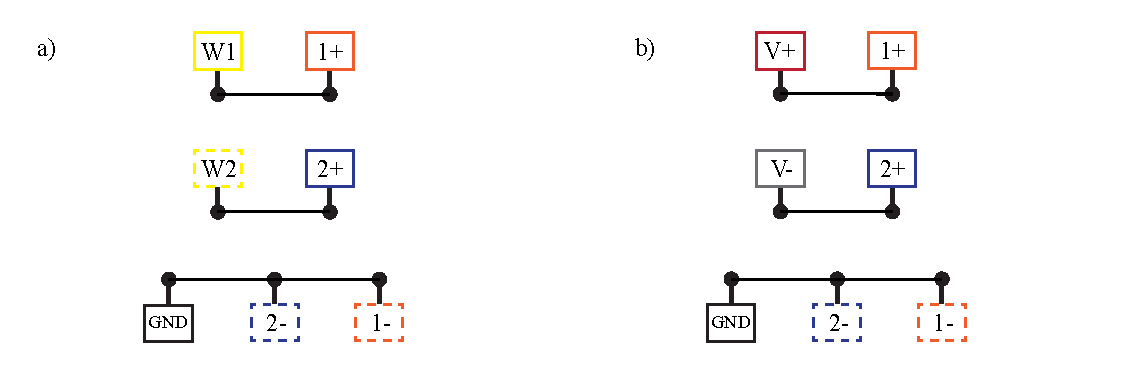
\includegraphics[width=1\textwidth]{Lab1-WavegenScopeConnections.pdf}
	%\caption{Circuit diagram for connecting the wavegen outputs to the scope probes (a) and connection the power supplies to the scope probes (b). Note that the scope probe negative terminals, indicated with a dashed line in the diagram and a white strip on the Analog Discovery wire, must be tied to the Analog Discovery ground. Also, the negative power supply wire is white on the Analog Discovery and has been indicated by gray box in the Figure. } \label{fig:WavegenScopeConnections}
%\end{figure}
%
%
%\begin{enumerate}
	%\item Use the Wavegen to generate a 10 kHz sine wave with an amplitude of 2 V, an offset of 0 V, a symmetry of 50\% and a phase of 0 degrees. Connect the output of the Wavegen on the Analog Discovery to the scope probes and measure the results using the Scope tool as shown in \hyperref[fig:WavegenScopeConnections]{Figure \ref*{fig:WavegenScopeConnections} (a)} and choose an appropriate time base and voltage range; display at least one period but no more than three periods.
	%\item Label the sine wave appropriately and then export an image of the Scope screen. Go to \textbf{File} -> \textbf{Export} and then set the \textbf{Source} to \textbf{Acquisition}. Click save and then choose an appropriate name and location for file. For the lab check, images must be shown to the lab instructor for accuracy. \label{itm:singlesine}
	%\item Using the same signal on channel 1, generate a second sine wave on channel 2 in the Wavegen that is 180 degrees out of phase. Remember to wire up the second Wavegen and Scope channels. 
	%\item On the scope, display channel 1, 2, and add a simple math channel that plots Channel 1 - Channel 2. Again, choose the appropriate time, voltage scales, and label the traces appropriately. Save an image of the Scope acquisition. \label{itm:dualsine}
	%\item Wire up the Analog Discovery so that the variable power supplies on the Analog Discovery are connected to the scope probes as shown in \hyperref[fig:WavegenScopeConnections]{Figure \ref*{fig:WavegenScopeConnections} (b)}. Set the power supplies to +5 V and -5 V (Analog Discovery 1 is fixed at +/-5 V while the Analog Discovery 2 has variable supplies). Display the results on the Scope and save an image with the appropriate labels and voltage scale. \label{itm:voltagerefs}
	%\item Reconnect the Wavegen to the scope probes as shown in \hyperref[fig:WavegenScopeConnections]{Figure \ref*{fig:WavegenScopeConnections} (a)} and generate a 100 kHz square wave with a 1 V amplitude, 1 V offset, symmetry of 50\%, 0 degree phase offset. Choose a time base that displays at least 1 period but no more than 3 periods. Also, set the trigger level so that the trace does not ``run''. Save an image of the acquisition. \label{itm:squarewave}
	%\item Add two X cursors, \textbf{View} -> \textbf{Cursors} -> X \textbf{Cursors}, and confirm that the period corresponds to a 100 kHz signal. Similarly, add two Y cursors and confirm that the peak-to-peak voltage is 2 V. Save an image of the scope showing the X and Y cursors (set the source to Scope instead of Acquisition). \label{itm:cursors}
%\end{enumerate}
%
%\section{Discussion Questions}
%
%Typically this would be where the discussion quires are located associated with the lab but for lab 1 there is no report and therefore no discussion questions.
%
%\section{Lab Check}
%
%All students must check out of the lab and the lab instructor the following items. Usually they are images from the lab, tables of values, completed circuits, etc..
%
%\begin{enumerate}
	%\item \hyperref[itm:singlesine]{Item \ref*{itm:singlesine}} - Single sine wave plot.
	%\item \hyperref[itm:dualsine]{Item \ref*{itm:dualsine}} - Dual sine wave plot.
	%\item \hyperref[itm:voltagerefs]{Item \ref*{itm:voltagerefs}} - Reference voltages plot.
	%\item \hyperref[itm:squarewave]{Item \ref*{itm:squarewave}} - Square wave plot.
	%\item \hyperref[itm:cursors]{Item \ref*{itm:cursors}} -  Square wave with cursors plot.
%\end{enumerate}
%
%\section{Lab Practical Exam}
%
%Once the lab check is completed you can complete the lab practical exam. The lab instructor will ask you to generate and display a variety of signals. The exam is pass or fail and it can be repeated as many times as necessary until the lab session ends. 
%
